\appendix

\section{Appendix: Original Twitter15/16 Benchmark Results}

This appendix preserves the fuller Twitter15/16 benchmark results that motivated the earlier version of the thesis. In the revised main text, Twitter15/16 are summarized as a comparative benchmark rather than treated as the primary empirical setting. To avoid losing the original benchmark detail, I retain the core benchmark figures here.

\subsection{Primary Benchmark Curves}

Figure~\ref{fig:app_twitter_veracity} and Figure~\ref{fig:app_twitter_reach} report the original Twitter15/16 size-based primary curves. These figures correspond to the benchmark values summarized in the main text: veracity peaking around AUC $=0.657$ at $k=20$ and reach peaking around $R^2=0.719$ at $k=180$ under the interaction-full specification.

\begin{figure}[htbp]
  \centering
  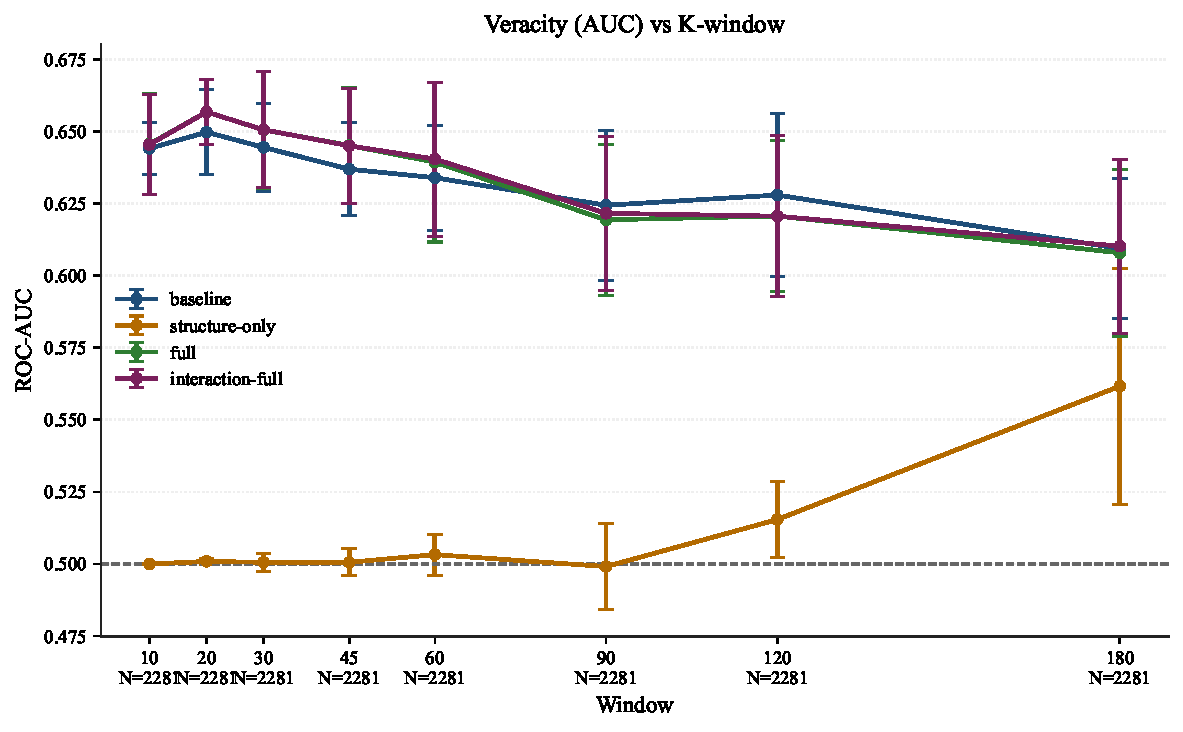
\includegraphics[width=0.82\linewidth]{Paper_sections/figures/TW_F1K_k_veracity_primary.pdf}
  \caption{Original Twitter15/16 benchmark veracity (AUC) across size-based windows. This was the main veracity figure in the earlier benchmark-centered version of the analysis.}
  \label{fig:app_twitter_veracity}
\end{figure}

\begin{figure}[htbp]
  \centering
  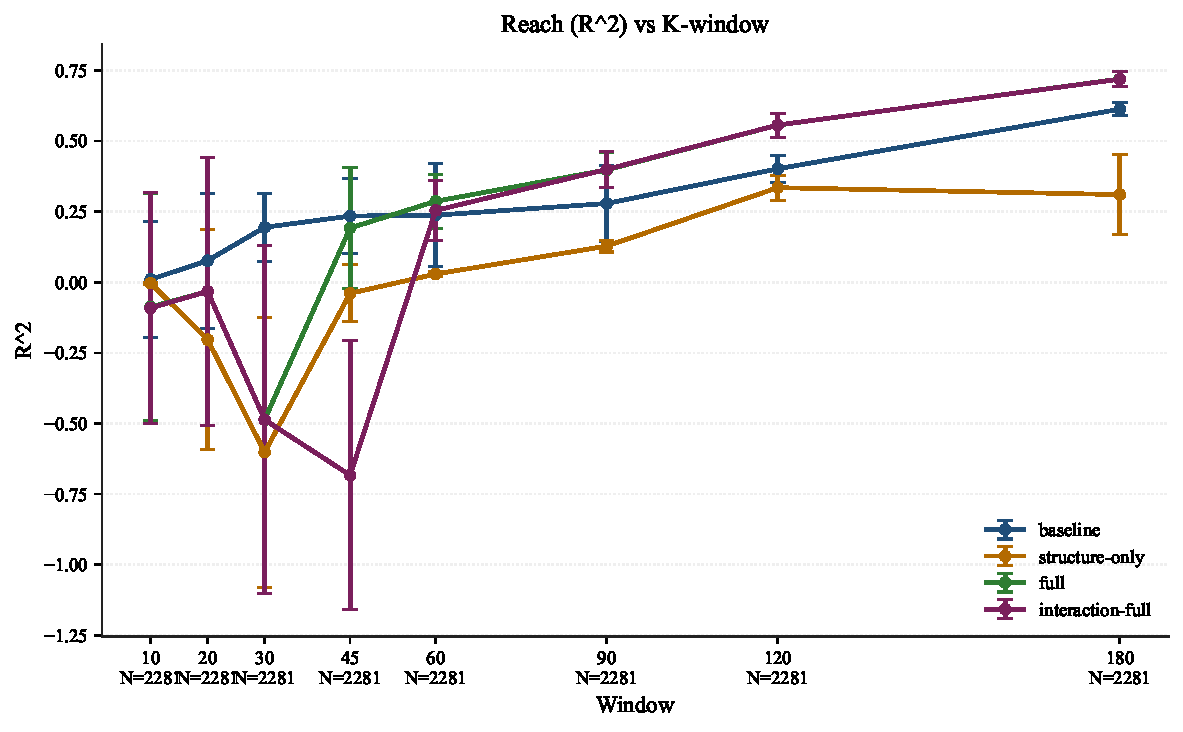
\includegraphics[width=0.82\linewidth]{Paper_sections/figures/TW_F2K_k_reach_primary.pdf}
  \caption{Original Twitter15/16 benchmark reach prediction ($R^2$) across size-based windows. This was the main reach figure in the earlier benchmark-centered version of the analysis.}
  \label{fig:app_twitter_reach}
\end{figure}

\subsection{Model Family and Signal Validation}

The benchmark pattern in model-family comparisons and permutation checks is also retained here. As in the main text, the benchmark suggests a moderate veracity signal and a stronger reach signal, with tree-based regressors contributing more clearly on the reach side.

\begin{figure}[htbp]
  \centering
  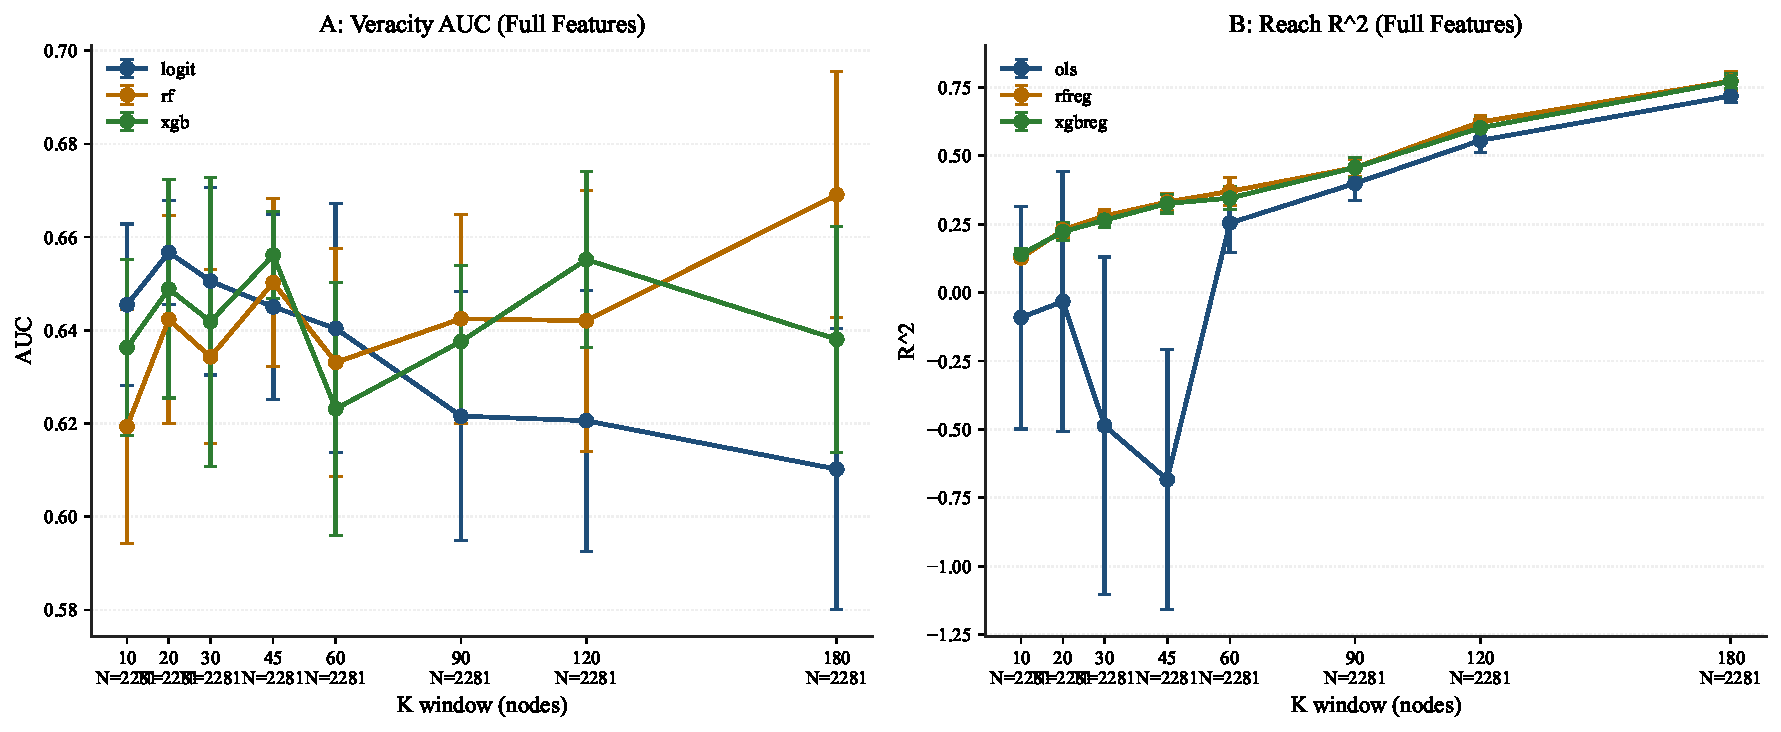
\includegraphics[width=0.9\linewidth]{Paper_sections/figures/TW_F3_model_family_full_only.pdf}
  \caption{Original Twitter15/16 benchmark model-family comparison under the full feature bundle.}
  \label{fig:app_twitter_model_family}
\end{figure}

\begin{figure}[htbp]
  \centering
  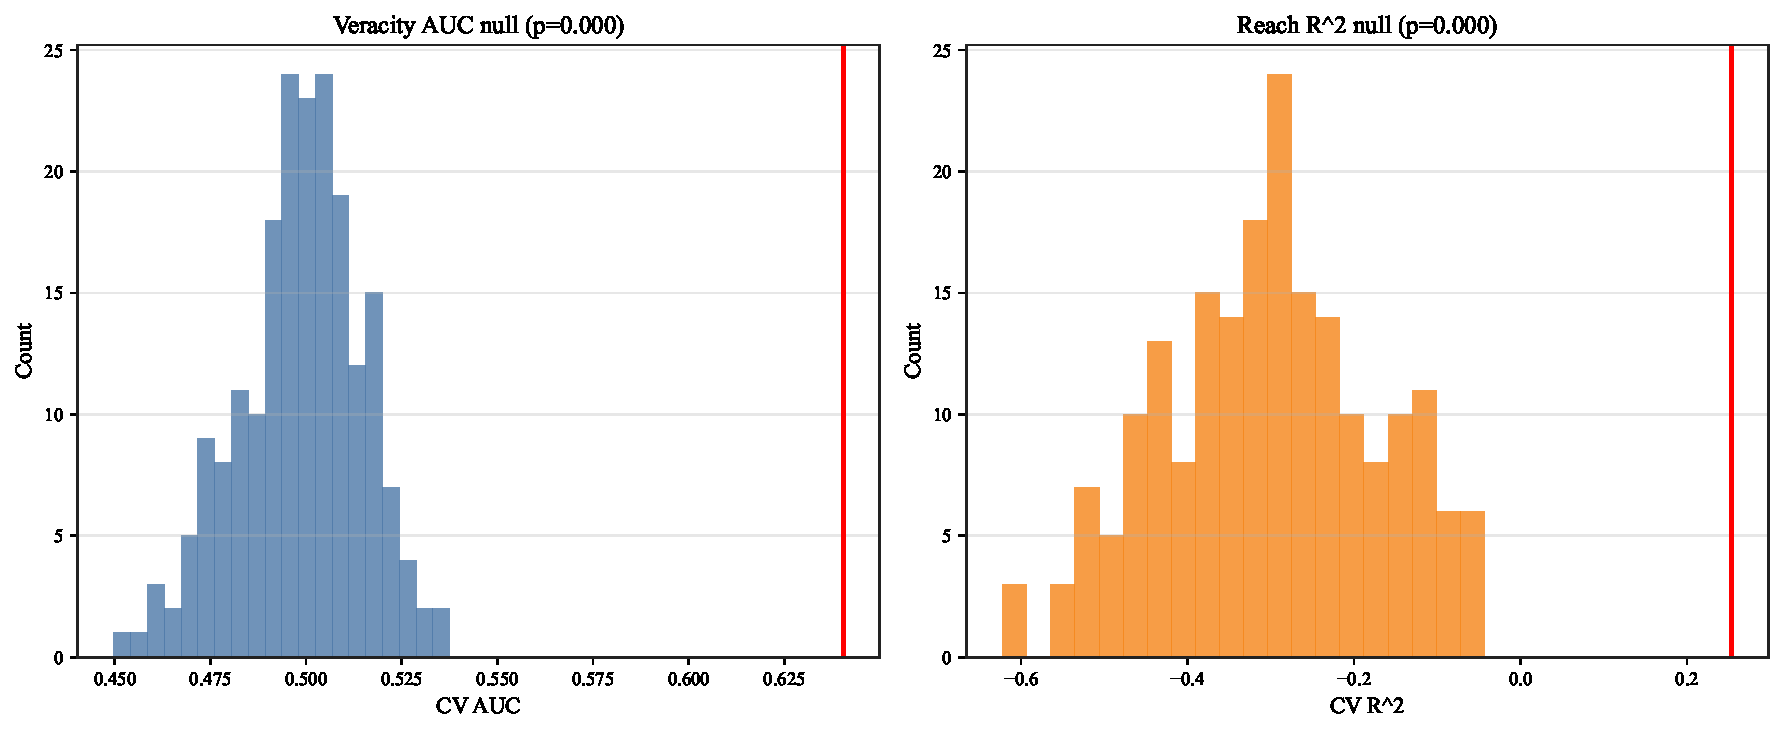
\includegraphics[width=0.88\linewidth]{Paper_sections/figures/TW_F5_permutation_test_signal.pdf}
  \caption{Original Twitter15/16 benchmark permutation tests at $k=60$. Both tasks separate clearly from the null in the benchmark setting, though the reach/veracity asymmetry remains visible.}
  \label{fig:app_twitter_perm}
\end{figure}

\subsection{Supplementary Time-Window Benchmark Figure}

For completeness, Figure~\ref{fig:app_twitter_time} retains the original benchmark time-window learning curve that was used as a supplementary check in the benchmark-centered version of the project.

\begin{figure}[htbp]
  \centering
  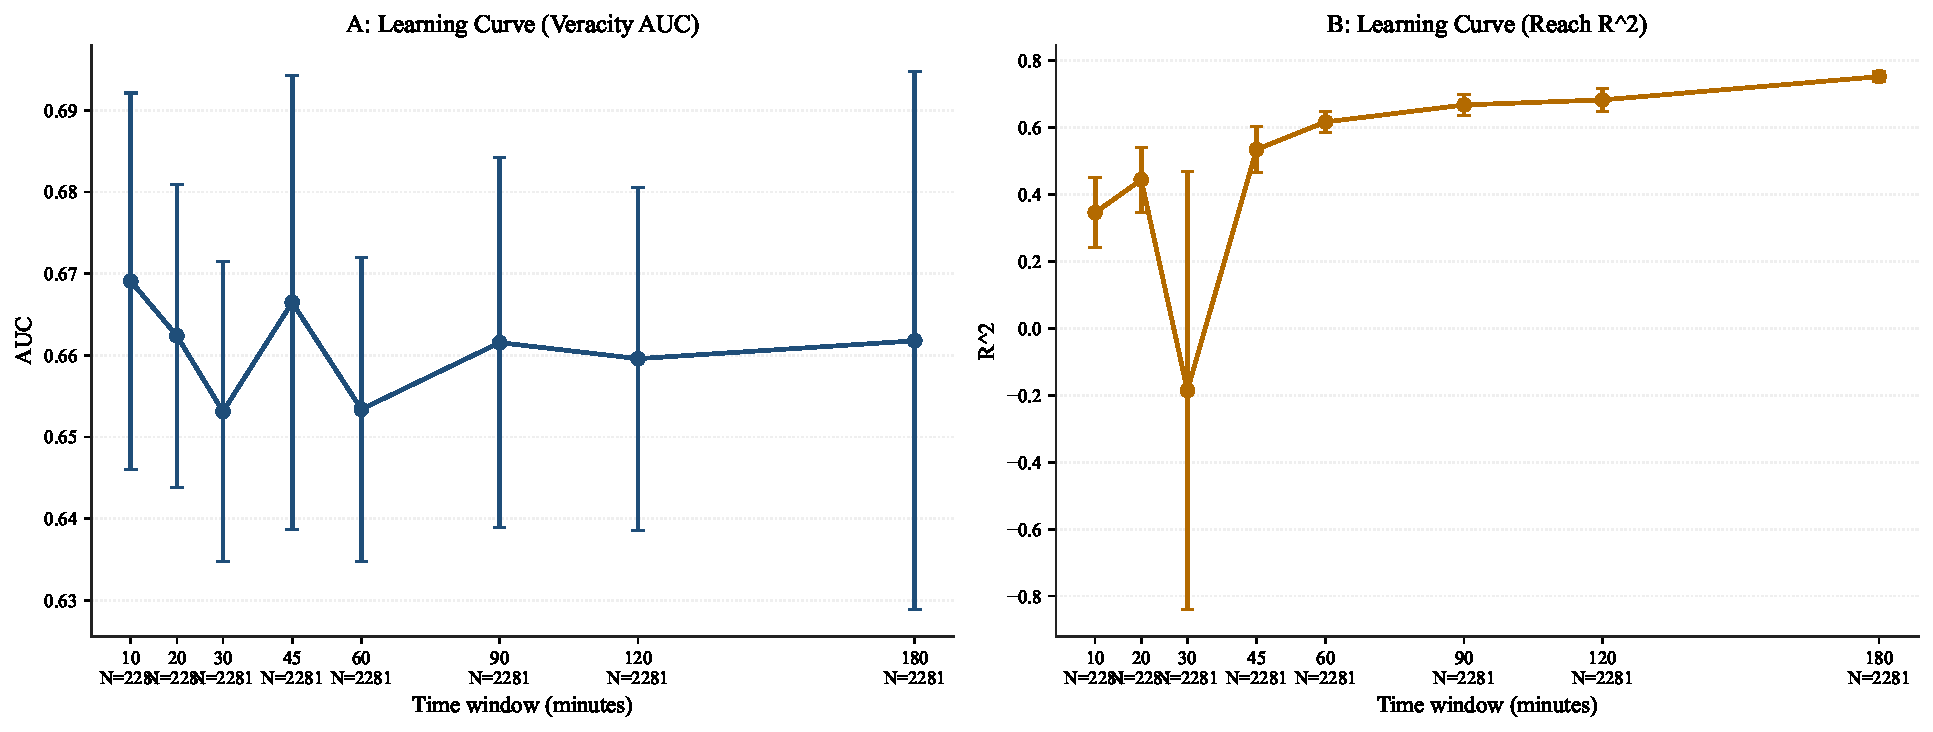
\includegraphics[width=0.88\linewidth]{Paper_sections/figures/TW_F6_learning_curve_time.pdf}
  \caption{Original Twitter15/16 benchmark time-window learning curve. In both the earlier benchmark-centered analysis and the revised FibVID-centered thesis, time windows remain supplementary rather than the primary design.}
  \label{fig:app_twitter_time}
\end{figure}
